\documentclass{article}

\usepackage{amsmath, mathrsfs, amssymb, stmaryrd, cancel, relsize,tikz,amsthm}
\usepackage{hyperref}
\theoremstyle{plain}
\newtheorem{theorem}{Theorem}[section]{\bfseries}{\itshape}
\newtheorem{proposition}[theorem]{Proposition}{\bfseries}{\itshape}
\newtheorem{definition}[theorem]{Definition}{\bfseries}{\upshape}
\newtheorem{lemma}[theorem]{Lemma}{\bfseries}{\upshape}
\newtheorem{corollary}[theorem]{Corollary}{\bfseries}{\upshape}
\newtheorem{exercise}[theorem]{Exercise}{\bfseries}{\upshape}

\theoremstyle{definition}
\newtheorem{example}[theorem]{Example}{\bfseries}{\upshape}

\newcommand{\tvs}{\textvisiblespace}
\newcommand{\ra}{\rightarrow}
\newcommand{\la}{\leftarrow}
\newcommand{\co}{\mathbf{code}}


\title{ITCS 532 Foundations of Computer Science\\
Class 3 - Universal Turing Machines}
\author{Rob Egrot}
\date{}

\begin{document}
\maketitle

\subsection{Universal Computation}
Machines for computation have existed for thousands of years. For example, the Antikythera mechanism dates back to the 1st or 2nd century BC, and was used by Ancient Greek astronomers to predict astronomical phenomena such as eclipses. The creation of programs to run on other devices also has a long history. The Banu Musa brothers, for example, invented in 9th century Persia an automatic machine for playing the flute that could be programmed to play different melodies. What distinguishes computers in the modern sense from these early machines is the concept of universal computation. That is, modern computers are able to simulate each other. We could, if we wanted, program a computer to perform the calculations of something like the Antikythera mechanism, or to imitate the Banu Musa brothers' flute player, but we could not, on the other hand, program the mechanical flute player to run Microsoft Windows. 

The first `true' computer (what we will call \emph{universal} computers) is thought to be Charles Babbage's Analytical Engine, designed, with significant contributions from Ada Lovelace, in 1837. This was an entirely mechanical device capable of performing arithmetic calculations and with flow control in the form of conditional branching and looping. This machine was never built due to the significant engineering challenge it posed. For reference, the Difference Engine no. 2, a simpler, non-universal, calculating engine designed by Babbage before the Analytical Engine was over 3 meters long and weighed 2.6 tons when it was finally built in 2002 (see Figure \ref{DE2}). 


\begin{figure}[ht]
\centering
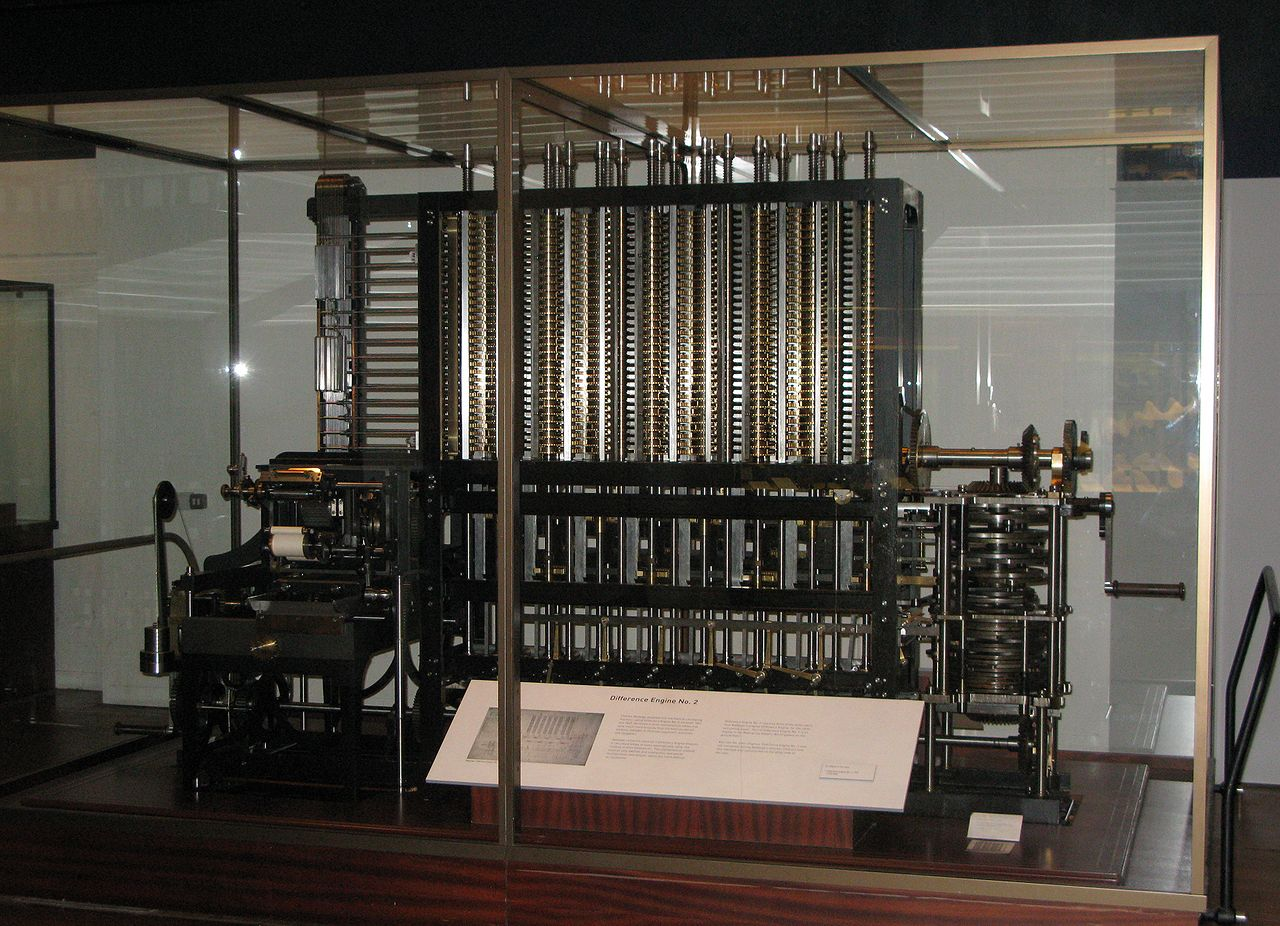
\includegraphics[scale = 0.22]{DE2.jpg}  
\caption{The Difference Engine no. 2. Photo from Wikipedia (https://commons.wikimedia.org/w/index.php?curid=4807331)}
\label{DE2}
\end{figure}

The remarkable thing about the Analytical Engine is that it \emph{could}, in theory, run Windows, though extremely slowly. While Babbage and Lovelace are possibly the first people to design a `modern' computer (in function, if not in form), they did not have the theoretical framework to fully understand what made their idea so revolutionary. The formalism of Turing machines provides this framework for us, and this is what we will explore in this section.  



\subsection{Encoding Turing Machines}
Remember that a Turing machine is defined by a $5$-tuple $(Q,\Sigma,q_0,H,\delta)$. Each part of this is finite. When we've been defining Turing machines we've been defining alphabets and states on an ad hoc basis. For example, we say things like ``let $\Sigma=\{a,b\}$'', or ``let $\Sigma=\{1,*\}$". When we choose an alphabet for a Turing machine the actual symbols we choose aren't important. For example, we could design equivalent machines using $\{a,b\}$ and $\{1,*\}$ as alphabets, by just, for example, assigning $a$ and $1$ the same meaning, and doing the same for $b$ and $*$. What this means is that the important thing about the alphabet a Turing machine works over isn't the symbols themselves, but just the number of distinct symbols. Since every TM uses only a finite number of symbols in its alphabet, if we have a countably infinite pool of symbols, let's say $\hat{\Sigma}=\{\sigma_0,\sigma_1,\sigma_2,\ldots\}$, then every TM is equivalent to one whose alphabet is a finite subset $\{\sigma_0,\ldots,\sigma_n\}$ of symbols from $\hat{\Sigma}$. We will need to include the special symbols $\tvs$ and $:$ in $\hat{\Sigma}$ too, and also the $\la$ and $\ra$ symbols for tape head control.

Similarly, though we gave the states in our machines arbitrary names sometimes, the important thing is just the number of different states and their roles in the computations. So we can fix $\hat{Q}=\{q_0,q_1,q_2,\ldots\}$ and then every TM is equivalent to one whose states are taken from $\hat{Q}$. 

Given a TM defined by $(Q,\Sigma,q_0,H,\delta)$ we can assume $Q$ is a finite subset of $\hat{Q}$, $\Sigma$ is a finite subset of $\hat{\Sigma}$, $q_0$ is just $q_0$ from $\hat{Q}$, and $:$, $\tvs$, $\la$, and $\ra$ are $\sigma_0$, $\sigma_1$, $\sigma_2$, and $\sigma_3$ from $\hat{\Sigma}$ respectively. Since we can now think of every TM as drawing from a fixed, countable pool of symbols, and since every part of the definition of a TM is finite, a Turing machine is specified by a finite subset of $\hat{Q}\cup\hat{\Sigma}$, along with a transition function $\delta$ that is formally a finite subset of $\hat{Q}\times\hat{\Sigma}\times\hat{Q}\times\hat{\Sigma}$. So the set of all Turing machines corresponds to a subset of the set of all finite subsets of a countable set, and so is countable. In other words there is a 1-1 function $\co$  from the set of all Turing machines to $\{0,1\}^*$. There are lots of ways we can define this function, and we give one example below.

\begin{itemize}
\item For $q_n$ we define $\co(q_n)$ to be $n+1$ `1' symbols. So, e.g. $\co(q_2)=111$.
\item For $\sigma_n$ we define $\co(\sigma_n)$ to be $n+1$ `1' symbols. So, e.g. $\co(\sigma_1)=11$. This is the same as the definition for $q_n$, but this isn't a problem because when we build up $\co$ to apply to whole Turing machines, the coded forms of states and symbols will be differentiated by their relative positions.
\item Given a Turing machine $T$ with states $Q=\{q_0,\ldots,q_m\}$ and alphabet $\Sigma=\{\sigma_0,\ldots,\sigma_n\}$ we define the strings 
\begin{equation*}\co(Q)=\co(q_0)0\co(q_1)0\ldots0\co(q_m)0\end{equation*}
and
\begin{equation*}\co(\Sigma)=\co(\sigma_0)0\co(\sigma_1)0\ldots0\co(\sigma_n)0\end{equation*}
\item Let $q_i$ be the accept state of $T$, and let $q_j$ be the reject state (we can safely assume that $T$ has these and only these halt states). The concatenated string $\co(Q)0\co(\Sigma)0\co(q_i)0\co(q_j)0$ encodes the states and alphabet that define $T$, so all that is left is to find a way to encode $\delta$.
\item $\delta$ is formally defined as a set of tuples $(q,\sigma,q',\sigma')$. We can code a tuple $t=(q,\sigma,q',\sigma')$ as 
\begin{equation*}\co(t)=\co(q)0\co(\sigma)0\co(q')0\co(\sigma')0\end{equation*} 
\item If $\delta$ is defined by tuples $t_1,t_2,\ldots,t_k$ we can define 
\begin{equation*}\co(\delta)=\co(t_1)\co(t_2)\ldots \co(t_k)\end{equation*}
\item Combining all this we can encode $T$ with 
\begin{equation*}\co(T)= \co(Q)0\co(\Sigma)0\co(q_i)0\co(q_j)0\co(\delta)\end{equation*}
\item If $I$ is a string defined by $I=\sigma'_1\sigma'_2\ldots\sigma'_l$ (where the $\sigma'$ are symbols from $\hat{\Sigma}$) we can encode $I$ using 
\begin{equation*}\co(I)=\co(\sigma'_1)0\co(\sigma'_2)0\ldots 0\co(\sigma'_l)\end{equation*}
\item We can encode the pair $(T,I)$ representing the Turing machine $T$ and input $I$ using 
\begin{equation*}\co(T,I)=\co(T)00\co(I)\end{equation*}
\end{itemize}   

The general idea is that strings of 1's represent symbols and states, and 0's are used as separators to indicate where the representation of one aspect of the TM ends and the representation of another part begins.

Consider as an example the Turing machine $T$ with alphabet $\Sigma=\{:,\tvs,a,b\}$ that just adds the symbol $a$ to the end of its input.

\begin{center}
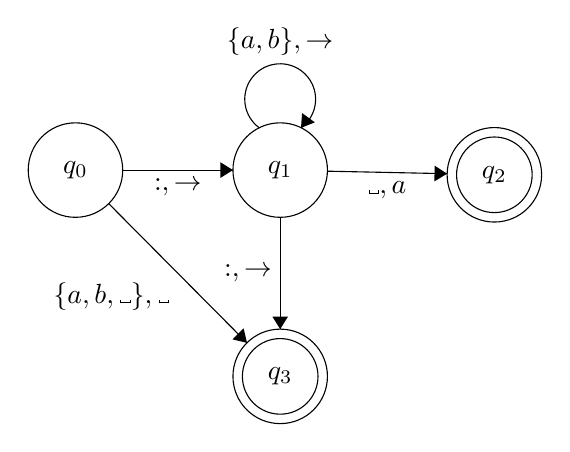
\begin{tikzpicture}[scale=0.2]
\tikzstyle{every node}+=[inner sep=0pt]
\draw [black] (9.4,-31.3) circle (3);
\draw (9.4,-31.3) node {$q_0$};
\draw [black] (22.4,-31.3) circle (3);
\draw (22.4,-31.3) node {$q_1$};
\draw [black] (36,-31.6) circle (3);
\draw (36,-31.6) node {$q_2$};
\draw [black] (36,-31.6) circle (2.4);
\draw [black] (22.4,-44.4) circle (3);
\draw (22.4,-44.4) node {$q_3$};
\draw [black] (22.4,-44.4) circle (2.4);
\draw [black] (12.4,-31.3) -- (19.4,-31.3);
\fill [black] (19.4,-31.3) -- (18.6,-30.8) -- (18.6,-31.8);
\draw (15.9,-31.8) node [below] {$:,\ra$};
\draw [black] (25.4,-31.37) -- (33,-31.53);
\fill [black] (33,-31.53) -- (32.21,-31.02) -- (32.19,-32.02);
\draw (29.17,-32.01) node [below] {$\tvs,a$};
\draw [black] (22.4,-34.3) -- (22.4,-41.4);
\fill [black] (22.4,-41.4) -- (22.9,-40.6) -- (21.9,-40.6);
\draw (21.9,-37.85) node [left] {$:,\ra$};
\draw [black] (11.51,-33.43) -- (20.29,-42.27);
\fill [black] (20.29,-42.27) -- (20.08,-41.35) -- (19.37,-42.05);
\draw (15.38,-39.33) node [left] {$\{a,b,\tvs\},\tvs$};
\draw [black] (21.077,-28.62) arc (234:-54:2.25);
\draw (22.4,-24.05) node [above] {$\{a,b\},\ra$};
\fill [black] (23.72,-28.62) -- (24.6,-28.27) -- (23.79,-27.68);
\end{tikzpicture}
\end{center}

The accept state is $q_2$, and the reject state is $q_3$. To encode this machine we first assign $a$ and $b$ correspondents in $\hat{\Sigma}$. We'll say $a=\sigma_4$ and $b=\sigma_5$ (because $:=\sigma_0$, $\tvs=\sigma_1$, $\la=\sigma_2$, and $\ra=\sigma_3$). The transition function $\delta$ is then defined by the tuples:
\begin{align*}
(q_0,:,q_1,\ra)&=(q_0,\sigma_0,q_1,\sigma_3)\\
(q_0,\tvs,q_3,\tvs)&=(q_0,\sigma_1,q_3,\sigma_1)\\
(q_0,a,q_3,\tvs)&=(q_0,\sigma_4,q_3,\sigma_1)\\
(q_0,b,q_3,\tvs)&=(q_0,\sigma_5,q_3,\sigma_1)\\
(q_1,:,q_3,\ra)&=(q_1,\sigma_0,q_3,\sigma_1)\\
(q_1,a,q_1,\ra)&=(q_1,\sigma_4,q_1,\sigma_3)\\
(q_1,b,q_1,\ra)&=(q_1,\sigma_5,q_1,\sigma_3)\\
(q_1,\tvs,q_2,a)&=(q_1,\sigma_1,q_2,\sigma_4)\\
\end{align*}

So using our definitions we get 
\begin{itemize}
\item $\co(Q)=10110111011110$
\item $\co(\Sigma)=101101110111101111101111110$
\item $\co(q_i)=111$
\item $\co(q_j)=1111$
\item Finally \begin{align*}\co(\delta)=&1010110111101011011110110101111101111011010 \\
                                        &1111110111101101101011110110110111110110111 \\
																				&101101111110110111101101101110111110\end{align*}
\item And so \begin{align*} \co(T)=     &1011011101111001011011101111011111011111100 \\
                                        &1110111101010110111101011011110110101111101\\
																				&1110110101111110111101101101011110110110111\\
																				&110110111101101111110110111101101101110111110                                    																
                                       \end{align*}
\end{itemize}

Because the codes of TMs using this method have a rigid pattern, it's conceptually straightforward to check whether a string is the encoded form of a Turing machine, and it's similarly straightforward to check whether a string is the coded form of a Turing machine along with an input. Specifically, the coded forms of TMs and inputs will follow the pattern \emph{declare states}00\emph{declare symbols}00\emph{declare halt state}0\emph{define transition function}00\emph{input}. Each declaration also has specific syntax which is easily checkable, and of course the declared states, symbols and transition function must all match up properly (e.g. the transition function can't use undeclared states and symbols etc.).

Note that strictly speaking $\co$ isn't a well defined function because it depends on how we write the transition function $\delta$. So the same TM could have different coded forms depending on what order we present the tuples from $\delta$. To solve this problem we can specify an order for writing out the tuples of $\delta$, but we don't need to get into the details of that here. If you check you will see that in the example above the tuples are not listed in alphabetical order. Technically this is a mistake, but we will not worry about this, either here or in the exercises. If we were actually trying to implement a coding system for real, then we'd have to be more careful.  


\subsection{Universal Turing Machines}
Since we can code Turing machines and inputs as finite strings over the alphabet $\{0,1\}$, it is possible to create Turing machines that manipulate these strings. We're interested in a very special kind of Turing machine that can take the coded form of another TM and an input and \emph{simulate} the action of that TM on the input. A Turing machine that can do this with the coded forms of other TMs and their inputs is called \emph{universal}. More precisely, if $U$ is a universal Turing machine (UTM), $T$ is any other TM, and $I$ is an input for $T$, then $U(\co(T,I))$ halts if and only if $T(I)$ halts (and accepts or rejects appropriately), and the output of $U(\co(T,I))$ is the coded form of the output of $T(I)$.

We'll sketch the design of a UTM in a moment, but before that we should realize that universal Turing machines are not strange to us in the 21st century. For example, the computer I wrote these notes on is universal. It can be given coded forms of abstract computation devices (programs) and simulate them on inputs, and this is all universal computation is (although real world universal computers are subject to memory limitations that abstract UTMs are not). The OS of a computer is a program being run over the basic architecture of the system, and the same architecture can support other operating systems too. And the OS itself runs other programs, which may themselves be capable of running other programs, so there are many layers of simulation taking place on a typical home computer.  

Anyway, we now present a rough sketch of how a UTM might work. Our design is for a 3-tape machine to keep things relatively simple. Of course we know that anything we can compute on a 3-tape machine can also be computed on a suitable 1-tape machine.

\begin{itemize}
\item The 1st tape is used for input and output. It starts with $\co(T,I)$ written on it (where $T$ is the machine to be simulated on input $I$). Later in the calculation it will store the state of the tape of $T$ in coded form.
\item The 2nd tape will be used to store $\co(T)$ for reference.
\item The 3rd tape will be used to store the coded form of the state of $T$.
\end{itemize} 

A run of this machine $U$ on input $\co(T,I)$ starts as follows:
\begin{enumerate}
\item $U$ copies $\co(T)$ from tape 1 onto tape 2.
\item $U$ erases $\co(T)$ from tape 1 and shifts $\co(I)$ to the start of the tape so tape 1 just contains $\co(I)$.
\item $U$ writes $\co(q_0)$ on tape 3.
\end{enumerate}

The simulation of a single step of $T(I)$ by $U$ goes as follows:

\begin{enumerate}
\item $U$ searches tape 2 for an instruction corresponding to the state of the machine coded on tape 3 and the symbol currently being read in coded form on tape 1. We need some method for defining which symbol is being read as tape 1 contains the input in coded form. One method we could use is to note that the coded forms of symbols are separated by 0's, so we can define the symbol being read as the one to the left of the 0 being read by the tape head. We just need to manage the tape head on tape one so it ends every simulated step reading a 0.
\item Based on the instruction it updates tape 3 to represent the new state of $T$, and updates tape 1 to represent the new contents of the tape of $T$ and the new position of the tape head.
\item If $T$ has reached a halt state then $U$ halts in the corresponding halt state, otherwise $U$ goes back to 1.
\end{enumerate}


\subsection{Are There Undecidable Problems?}
We claimed in the first class that there are decision problems that cannot be solved by a Turing machine. We will now prove this is true using an abstract argument. In the next class we'll give some specific examples. First remember that every decision problem corresponds to a formal language (a subset of $\Sigma^*$ for some finite alphabet $\Sigma$). Given a finite alphabet $\Sigma$ the set of all finite strings over $\Sigma$, which we call $\Sigma^*$, is countably infinite. The formal languages over $\Sigma$ are the subsets of $\Sigma^*$, so the set of all formal languages over $\Sigma$ is $\wp(\Sigma^*)$, which is uncountable. 

On the other hand, we have just shown that every Turing machine can be represented by a finite string over the alphabet $\{0,1\}$. So the set of all Turing machines (where we count machines that make equivalent computations as being the same) is a subset of the set of all finite strings over $\{0,1\}$, i.e. $\{0,1\}^*$, which is countably infinite. 

So, the set of all Turing machines is countably infinite, but the set of all formal languages over a finite alphabet is uncountably infinite. So there must be (many) more formal languages (and so decision problems) than there are Turing machines capable of deciding them! We conclude that there are decision problems which cannot be decided (or semidecided) by a Turing machine. 

Now, you might first be surprised by this, but after thinking about it for a while you might think that this is to be expected. After all, by identifying formal languages with arbitrary subsets of the set of all finite strings  over the alphabet, we are opening the door for all kinds of strange, undefinable formal languages. So you might be optimistic that, though undecidable problems must exist (by the argument above), at least all the `natural', or `reasonably definable' languages are decidable. But this too is not true, as we shall see in Section \ref{S:und}. 


\subsection{Other Abstract Universal Computers}
It turns out that abstract universal computers are actually very common. Many if not most deterministic processes that are not obviously trivial turn out to be capable of universal computation, in the sense that you can decide rules for input and output that let you simulate Turing machines (including UTMS). 
\newline
\newline
\textbf{Rule 110}\\
An elementary cellular automaton consists of a 2-way infinite tape whose cells can contain either 0 or 1. At each step of a computation the contents of a cell changes based on its contents and the contents of its immediate neighbours. Rule 110 is an elementary cellular automaton with update rules described in the following table.

\begin{center}
\begin{tabular}{| c |c |c |c |c |c |c |c |c|}
\hline
 Cell configuration          & 111 & 110 & 101 & 100 & 011 & 010 & 001 & 000 \\\hline 
 New contents of center cell &  0  &  1  &  1  &  0  &  1  &  1  &  1  &  0\\ \hline   
\end{tabular}
\end{center}

It can be shown that Rule 110 is capable of universal computation. This is a rather vague statement, and it's not clear what it means. In what sense do elementary cellular automata even do `computations' at all? If we wanted to formally prove this assertion, we would have to carefully define concepts like `input', `output' `computation' for cellular automata. Roughly speaking, for a cellular automaton to be `universal' we must be able to define these concepts in such a way that, when the `input' corresponds to the code of a computable function $f$ and a string $I$, the `output' will correspond to the code of $f(I)$. The actual proof that this can be done for Rule 110 is due to Matthew Cook. The proof involves several detours through other forms of computation, and is rather complicated.

Note that Rule 110 can't halt, so we have to adjust the definition of `computation' a bit to take this into account.  
\newline
\newline
\textbf{Conway's Game of Life}\newline
The Game of Life, invented by John Conway, is another example of a cellular automaton, though in this case it is not elementary as it has an infinite grid rather than a single tape. Again each cell contains either 0 or 1. If a cell contains 1 then it is `live' and if it contains 0 then it is `dead'. The update rules are as follows:
\begin{enumerate}
\item A live cell with fewer than two live neighbours dies.
\item A live cell with two or three live neighbours stays live.
\item A live cell with four or more live neighbours dies.
\item A dead cell with exactly three live neighbours becomes live. 
\end{enumerate}

Given how much more complicated this is than Rule 110 it should come as no surprise that the Game of Life is also capable of universal computation, and indeed this is true. Industrious players have created systems for producing many kinds of behaviour within the Game, and you can play around with it at \url{https://bitstorm.org/gameoflife/}.
\newline
\newline
\textbf{Langton's Ant}\\
Langton's ant is essentially a Turing machine variant with an infinite 2D grid instead of a tape. Every square of the grid can be black or white. The `ant' is the tape head. The ant can face in four directions, up, down, left, and right. The movement of the ant is very simple. If the ant is in a white square it turns to the right, colours its square black, then moves forward one square. If the ant is in a black square it turns left, colours its square white, then moves forward one square. Despite its simple behaviour, Langton's ant is also capable of simulating any Turing machine, and so is capable of universal computation (though, like Rule 110 and the Game of Life, there is no way to halt, so we have to adjust the definition of `computation').

Despite the simple deterministic rules, the movements of the ant are often seemingly chaotic (to the human eye) at first, but all known starting configurations of the grid in Langton's ant lead to the ant eventually creating an orderly `highway' out to infinity in one direction. It is an open question whether this is true for all starting configurations. 

You can experiment with this at e.g. \url{https://sciencedemos.org.uk/langton_ant.php}

\end{document}